\chapter{Contributions}

\section{Modélisation}\label{sec:modelisation}
%traduction des patterns des réseaux de signalisations vers le formalisme des frappes de processus

%Ig------->PH
\subsection{Du Graphe d'Interaction(GI) au formalisme des frappes de processus}

Pour traduire notre réseau de signalisation en frappe de processus, nous avons identifié un ensemble de motifs dans le réseau de signalisation auxquels nous avons 
associé les motifs équivalents en frappe de processus. Le tableau \ref{tab:patterns} répertorie quelques exemples de motifs, leurs équivalents en frappes de processus et une brève 
description de leur sémantique. 

En plus de l'identification des motifs, nous avons défini un comportement pour chaque motif. Nous nous sommes inspiré de la sémantique de Thomas\cite{Thomas73}. Ainsi, si un composant est un activateur 
d'un autre composant, il va l'activer s'il est présent et l'inhiber s'il est absent. Réciproquement, si un composant est un inhiteur d'un autre composant, il va l'inhiber s'il est 
présent et le composant s'activera si son inhibiteur est absent. Nous avons en plus des cas simples modélisé les cas les plus complexes comme les décompositions des complexes, les
coopérations entre composants pour influencer la dynamique d'un autre composant et les synchronisations pour également 
influencer la dynamique d'un autre composant.

\begin{table}
\begin{tabular}{|c|c|M{4cm}|}
\hline
\textbf{(A) Les motifs Biologiques}

&

\textbf{(B)équivalents en frappes de processus}

&

\textbf{(C)Brèves descriptions}

\tabularnewline \hline
\begin{tikzpicture}[auto]
\path[use as bounding box] (-0.7,-0.3) rectangle (2.5,2);

\node[qgre] (a) at (0,1) {a};
\node[mod] (i) at (1,1) {i};
\node[qgre] (b) at (2,1) {b};
\node[es] (d) at (1,2) {Simple activation};

\path
 (a) edge[act] (i)
 (i) edge[st]  (b);
\end{tikzpicture}

&


\begin{tikzpicture}
\exphpatact
\end{tikzpicture}

&

Simple activation du composant b par le composant a


\tabularnewline \hline
\begin{tikzpicture}[auto]
\path[use as bounding box] (-0.7,-0.3) rectangle (2.5,2);

\node[qgre] (a) at (0,1) {a};
\node[mod] (i) at (1,1) {i};
\node[qgre] (b) at (2,1) {b};
\node[es] (d) at (1,2) {Simple inhibition};
\path
 (a) edge[inh] (i)
 (i) edge[st]  (b);
\end{tikzpicture}

&

\begin{tikzpicture}
 \exphpatini
\end{tikzpicture}

&

Simple inhibition du composant b par le composant a


\tabularnewline \hline

\begin{tikzpicture}[auto]
\path[use as bounding box] (-0.7,-0.3) rectangle (2.5,3);
\node[qgre] (a) at (0,2) {a};
\node[mod] (i) at (1,1) {i};
\node[qgre] (b) at (0,0) {b};
\node[qgre] (c) at (2,1) {c};
\node[es] (d) at (1,3) {activation or inhibition};

\path
 (a) edge[act] (i)
 (b) edge[inh] (i)
 (i) edge[st]  (c);
\end{tikzpicture}


&

\begin{tikzpicture}
 \exphpatai
\end{tikzpicture}

&

Activation ou inhibition du composant c soit par le composant a soit par le composant b

\tabularnewline \hline

\end{tabular}

\caption{\label{tab:patterns}
Exemples de motifs biologiques (voir colonne (A)) avec les équivalents en frappes de processus (voir colonne (B)) et une brève description de la dynamique sous jacente(voir colonne (C).
}

\end{table}

\subsection{Estimations des paramètres temporels}\label{sec:estimations}
%estimation des paramètres temporelles
La prise en compte de l'aspect temporel et stochastique des réactions biologiques nous contraint à utiliser des paramètres qui 
vont nous permettre d'introduire ces aspects dans notre modèle pour raffiner davantage la dynamique du modèle et permettre de 
mieux capturer la dynamique du système que nous voulons étudier. 

Nous allons nous servir d'un paramètre(le taux) qui va permettre de définir à la fois la durée et la probabilité de survenue d'un évènement.
Le taux d'une action est une approximation de l'inverse  du temps moyen nécessaire pour l'exécution de cette action. L'idée est de faire 
en sorte que le temps moyen nécessaire pour jouer une action, corresponde à l'interval de temps qui sépare cette action de la précédente. Nous 
allons distinguer deux situations: (i) les noeuds ou composants du réseau pour lesquels nous n'avons pas de mesures et (ii) ceux pour lesquels
nous avons les mesures des séries temporelles.

Pour les molécules dont nous n'avons pas de mesures, nous allons choisir le même taux($10$) et le même facteur d'absortion de stochasticité($50$) pour jouer toutes 
les actions.

%Estimation des paramètres temporelles (t1 t2 t3 t4 t5 ...) pour les gènes 
Pour les autres, l'idée de l'estimation des paramètres temporels est de déterminer les différents instants de temps pour lesquels on considère un changement 
d'état à partir des niveaux d'expressions. La détermination des changements d'état va donc s'appuyer sur un choix au préalable des seuils qui 
vont déterminer les différents niveaux d'activités. Ainsi, dès que le niveau d'expression va traverser un seuil, on va considérer qu'il y a un 
changement d'état au niveau du composant. Ce qui doit donc se traduire par une action dans notre modèle qui va entrainer cette dynamique.

Dans un premier temps, nous devons donc déterminer les différents instants $t_{i}$ correspondants à un changement d'état. Par la suite nous devons 
donner les taux aux actions responsables de cette dynamique de façon à pouvoir les observer aux instants estimés.

%intégration des paramètres temporelles sous forme de rate et d'absorption de stochasticité ( r et sa)


%pour les autres molécules



\section{Comparaison des simulations avec les données}

\subsection{Simulation par sous-graphe}

Les premières simulations de notre modèle nous donnent des résultats assez compliqué à analyser. Pour simplifier l'analyse et mieux comprendre
la dynamique de notre modèle, nous nous sommes proposé de l'étudier par sous-graphe. L'idée est de décomposer notre graphe des insteractions en sous-graphes. 
Chaque sous-graphe est un ensemble de composants requis partant d'un gène dont nous voulons observer la dynamique  jusqu'au noeud d'entré du réseau. Nous avons 
ainsi pu analyser  la dynamique de notre réseau par sous-graphe. Nous avons commencé à reconstituer le graphe initial en mettant ensemble les sous-graphes pour
retrouver notre modèle initial(avant décomposition par sous-graphes). Pour terminer 
ce travail nous devons mettre en oeuvre le mécanisme de synchronisation entre les composants dans le formalisme des frappes de processus.


\subsection{Discrétisation des données de séries temporelles}\label{sec:discretisation}
%discretisation des données de séries temporelles
Les données de comparaison sont des données continues et nous voulons les comparer avec les résultats d'un modèle discret. Nous sommes par conséquent 
obligés de discrétiser les données de séries temporelles  pour avoir leur expression discrète afin de pouvoir aisément les comparer avec les résultats 
produits par les simulations de notre modèle.
Nous avons proposé un algorithme de discrétisation qui va prendre en entrée une série temporelle continue et  produire en sortie une série temporelle
discrète sur trois niveaux. L'algorithme \ref{alg:Discretization} détail le principe de la discretisation qui a été utilisé. Nous pouvons observer les résulats 
de la discrétisation en utilisant l'algorithme \ref{alg:Discretization} sur la figure \ref{fig:simulations}.
\begin{algorithm}
\caption{Discretization of experimental data}
\label{alg:Discretization}
\begin{algorithmic}
\REQUIRE $X$ a table of experimental data
\ENSURE $Y$ a table of discretized data
%\STATE $y \leftarrow initialState(x)$
\FORALL{ gene $i$ in $X$ } 

\STATE $threshold \leftarrow computeThreshold(X[i,]);$
\STATE $Y[i,0] \leftarrow initialState(threshold,X[i,]);$
\FORALL {$j$ in $numberExpression$}
  \IF{$Increase(X[i,j],X[i,j+1])$}
   \STATE $computeSignificativityOfIncrease(threshold,X[i,j],X[i,j+1]);$
   \STATE $fixeSTATE(Y[i,j],Y[i,j+1]);$
  \ELSE
   \STATE $computeSignificativityOfDecrease(threshold,X[i,j],X[i,j+1]);$
   \STATE $fixeSTATE(Y[i,j],Y[i,j+1]);$
  \ENDIF
\ENDFOR

\ENDFOR

\end{algorithmic}
\end{algorithm}

%simulations
\subsection{Simulations}\label{sec:simulations}
%préciser qu'il s'agit des sous graphes pour chaque gène

Dans cette section, nous présentons les résultats préliminaire de notre travail. La figure \ref{fig:simulations} nous donne les résultats de la discrétisation et 
de la simulation effectuée sur les sous-graphes de notre modèle pour trois gènes. Nous constatons que nous réussissons à reproduire la dynamique des gènes. De haut en bas,
les trois premier graphiques représentent les tracés des données des séries temporelles continues des trois gènes que nous avons choisi pour illustrer les résultats actuels.
Les trois graphiques suivants représentent les résultats obtenus en effectuant la discrétisation de chaque courbe continue. Enfin les trois derniers graphiques sont les 
courbes obtenues après simulation du modèle. En analysant ces résultats, nous constatons que le modèle permet de reproduire avec certes des imprécisions la dynamique des gènes.
L'aspect stochastique du modèle fait qu'il est difficile d'obtenir avec exactitude la dynamique voulue. Dans la prochaine section nous allons présenter quelques perspectives à ce 
travail.

\begin{figure}[p]
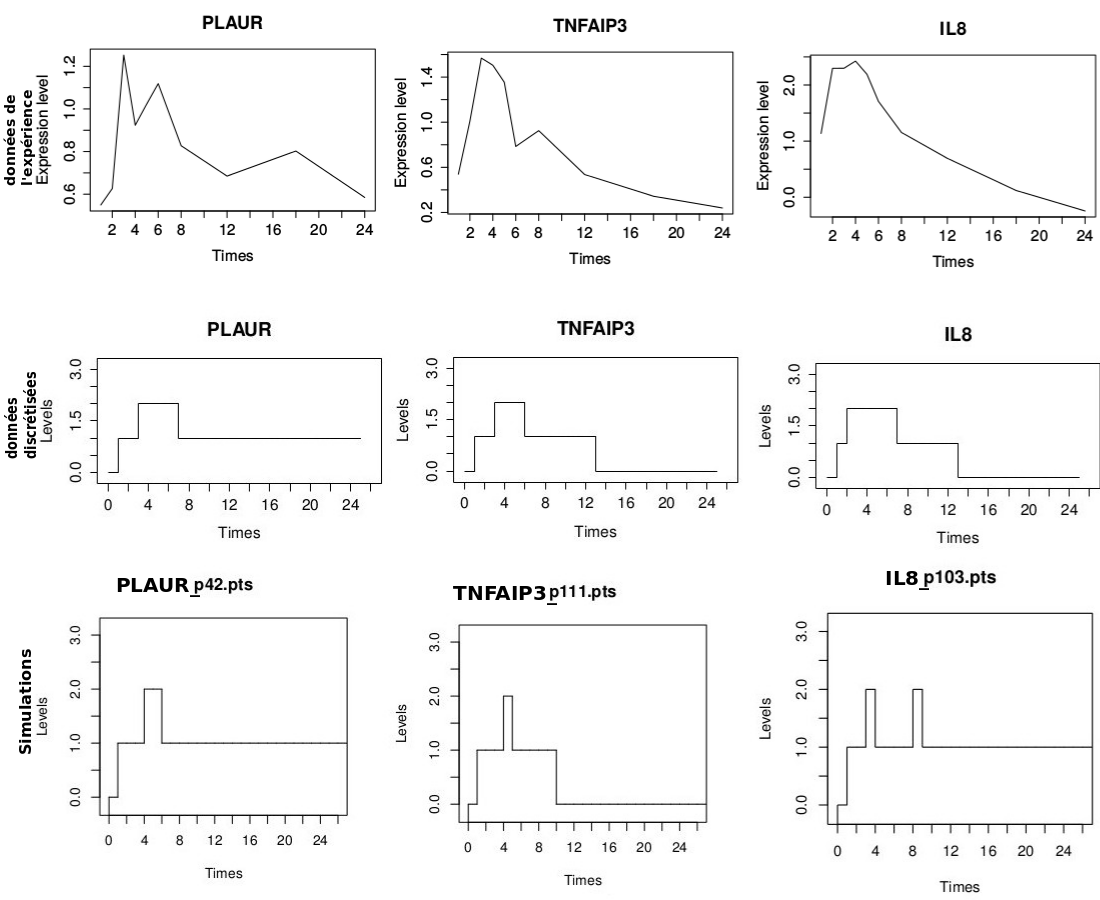
\includegraphics[scale=0.35]{images/courbe-cst1.png}
\caption{\label{fig:simulations}
Résultats de la discrétisation et de la simulation.
}
\end{figure}
